\chapter{Introduction to Mesquite} \label{sec:intro}

\section{Overview of Mesh Quality}

\hskip 0.25in {\it Mesh quality} refers to geometric properties of a mesh such as
local volume, smoothness, shape, and orientation that, if not properly
controlled,
can adversely affect solution accuracy or computational efficiency of numerical simulations. In this section we give an overview of the role of mesh quality
in the context of computer simulations of physical phenomena. \newline

Simulation of many phenomena in the physical world involves computing
numerical
solutions to partial differential equations (PDE's). Commonly used approaches
to computing  numerical solutions such as finite volume and finite
element methods require the use of approximations to the continuum operators
in the PDE and a mesh or grid to subdivide the physical domain into small
subregions. Together, the approximations and the mesh define a discretization.
The difference between the exact solution to the PDE and the numerical solution is known as the discretization error. A {\it convergent}
discretization means that the discretization error will asymptotically
approach zero as the characteristic mesh size ``h''
approaches zero. Decreasing mesh size to reduce discretization error to
nearly zero is often impractical in realistic simulations due to limited
computing resources. One way to increase the accuracy of simulations with the
same computer resources is to {\it adapt} the mesh to the domain and to the
numerical solution. In adaptive refinement, the local mesh volume (or size)
is made smaller in locations where the local discretization error is large and
is made larger in locations where the error is small. In local h-refinement,
mesh volume is made smaller by locally subdividing the mesh. In
r-refinement, mesh volume is made smaller by moving mesh nodes closer together.
Geometric adaptation can also be important in improving simulation accuracy. In regions of high domain curvature one adapts the mesh to the domain geometry by creating locally smaller mesh sizes. We see, then, that local mesh size (or volume) is a critical parameter in determining the accuracy of a simulation. \newline

Aside from local mesh size, several other geometric mesh properties can affect
solution accuracy. These include mesh smoothness, local mesh angles, aspect
ratio, and orientation. For example, in some discretization methods there will be a
loss of accuracy if the mesh is not smooth.  In other cases, aspect ratios and
orientation must be carefully adapted to the solution in order to maintain a
certain level of accuracy. Simulations using meshes or domains that evolve
in time (such as in ALE simulations) usually require that initially good
geometric mesh properties be retained throughout the simulation time period.
It is thus often important to control other geometric mesh properties in addition to local mesh size within an adaptive simulation. \newline

In addition to solution accuracy, geometric mesh properties can also affect the amount of computer time required to obtain the numerical solution. Simulation codes usually employ iterative solvers to solve systems of equations and thus obtain numerical solutions to PDE's. The rate at which these solvers converge is determined by the spectral radius of a certain matrix. The spectral radius of the matrix is affected by, among other things, geometric properties of the mesh. Poor mesh quality can thus adversely impact solution efficiency. \newline

Adaptive meshing techniques require an initial mesh to begin the adaptation procedure. Poor quality of the initial mesh (relative to the adapted mesh) can be difficult to overcome or, at least, reduce the efficiency of
the adaptive procedure. For example, if the initial mesh contains locally inverted elements, these can often be fixed before the adaptive procedure begins. As another example, if it is known \`{a} priori that small angles will be needed on the boundary of the domain to obtain reasonable simulation accuracy, one should try to first create the small angles in the initial mesh to improve the efficiency of the subsequent adaptive meshing procedure. \newline


Many simulations, particularly those in industry, are performed in a
non-adaptive setting. That is to say, an initial mesh is generated and
used throughout the calculation. The mesh is not changed as the solution
is computed. Mesh quality remains important for such calculations. First,
for complicated geometric domains it is often difficult to obtain good
initial mesh quality. This is particularly true for non-simplicial meshes
but can be true for simplicial meshes as well. A common requirement is that the mesh be smooth. Many simulation codes will not run to completion if the initial mesh contains a local volume which is negative. These must be eliminated before a simulation can begin. Analysts performing
non-adaptive calculations often have considerable experience in using a variety
of meshes on their problem and have a good \`{a} priori idea of what constitutes
good mesh quality for a given problem. They thus desire to control the usual
geometric mesh properties of the non-adapted mesh carefully.



\section{How Mesh Quality Is Improved}
Mesh quality can and should be considered during many stages of
the mesh generation process from de-featuring CAD models to
creation and adaptation of the mesh. Thus, for example, certain
non-essential features of a CAD model, if eliminated, would go a
long way to improving the quality of the mesh, depending upon
the meshing scheme. Other critical meshing parameters which can
affect mesh quality include geometric domain partitions, interval size
and count, interaction of meshes within large assemblies of parts,
biasing requirements, corner picking, etc. Choices made during the
mesh generation phase of an analysis may have a large impact on
initial mesh quality.  Mesh quality can thus be improved by changing the
way in which the domain is meshed. \newline

Once the meshing stage is completed, one can improve mesh quality
by techniques such as vertex movement and local topology modification.
In vertex movement schemes, one seeks to reposition existing mesh vertices to
achieve better quality. If vertex movement is undertaken within an adaptive
setting, it is commonly referred to as r-refinement.
Classic examples of vertex movement methods
include Laplace smoothing \cite{F88} and Winslow smoothing \cite{Winslow}.
It is helpful, in vertex movement schemes, to first be
able to measure mesh quality so that one can explain in what sense one
has improved it. Given a {\it metric} to measure mesh quality,
one can formulate a numerical
optimization problem which guides vertex movement to find the optimal
mesh and thus improve its quality.  Numerical
optimization methods recently
developed for unstructured meshes include \cite{Opt-MS,Kn00,FrKn01,
FeasNewt,bjoe:swap,bjoe:chain-swap,es92}. \newline
%We refer the reader to ref xxx
%which is a survey of mesh quality improvement methods which have appeared
%in the literature. \newline

A large number of mesh quality metrics have been devised to measure
mesh quality. Many of these metrics are independent of any solution
properties and are thus not useful in adaptive meshing. However, there
are a number of weighted quality metrics which can be tied to the
numerical solution via error indicators or other information for adaptive
meshing. \newline
%Examples of weighted metrics which have or could be used in
%adaptive calculations include those of Brackbill (ref), Knupp (ref), etc. \newline

Another way to improve mesh quality is to use local topological modification methods in which mesh vertices or elements are locally created and/or destroyed. These methods are very successful when applied to simplicial meshes, often within an adaptive context.  Local topology modification is less effective on non-simplicial meshes. \newline

Mesh quality improvement remains an important on-going research area.
There remain, for example, open questions with regard to metrics which
can be used in adaptive settings, theoretical questions on problem
formulation, and how to obtain improved meshes quickly. An important
subset of Mesquite capabilities is based on a mathematical theory that we
are developing which we call the Target-matrix paradigm (TMP).  The
basic idea is similar to that from Harmonic mappings, as applied to mesh
generation: use only a few very soundly formulated quality metrics and
adapt the mesh to a wide variety of specialized purposes via specification
of the mapping on the target manifold. However, TMP is formulated as a
discrete optimization problem, which allows direct control over important
properties such as invertibility which must hold even if the asympototic limit
is not reached. The mathematics behind the Target-matrix
paradigm can be found in \cite{formal,local2dmetrics,convexity,analysis2D,labelinv,labelinv-imr,tgtcons}. \newline

Although mesh quality improvement algorithms have been widely implemented
in both meshing and applications codes, it has always been difficult to
improve the quality of a mesh created in one software package using an
improvement algorithm which has been implemented in another.  This difficulty
and others have inspired the creation of the Mesquite software library.
This library is described in the next section. \newline


\section{Mesquite Goals}
Mesquite (Mesh Quality Improvement Toolkit) is designed to provide a
stand-alone, portable, comprehensive suite of mesh quality improvement
algorithms and components that can be used to construct custom quality
improvement algorithms.
The design is flexible so that the algorithms can be applied to many
different mesh element types and orders and referenced to both
isotropic and anisotropic ideal elements.  Mesquite provides a robust
and effective mesh improvement toolkit that allows both meshing
researchers application scientists to benefit from the latest
developments in mesh quality control and improvement. \newline

Mesquite design goals are derived from a mathematical framework and
are focused on providing a versatile, comprehensive, inter-operable,
robust, and efficient library of mesh quality improvement algorithms
that can be used by the non-expert and extended and customized by
experts.  In this section we highlight the current status of Mesquite
in several of our design goal areas. \newline


{\bf Versatile.}  Mesquite works on structured, unstructured, and
hybrid meshes in both two and three dimensions. The design permits
improvements to meshes composed of triangular, tetrahedral,
quadrilateral, hexahedral, prismatic (wedge) and pyramidal elements.
Support for general polyhedral elements may be added at a future time.
It currently incorporates
only methods for node movement; plans for topology modification and
hybrid improvement strategies lie in the future.  Node movement
strategies include both local patch-based iteration schemes for one or
a few free vertices and global objective functions which improve all
vertices simultaneously. Mesquite will be applicable to both adaptive
and nonadaptive meshing and to both low- and high-order discretization
schemes, but currently works with non-adaptive meshes containing
linear elements. \newline

{\bf Comprehensive.}  Mesquite will address a large variety of mesh
quality improvement goals including mesh volume control (sizing,
invertibility), mesh angles, aspect ratios, and orientation. Specific
goals include mesh untangling, mesh smoothing, shape improvement,
anisotropic smoothing, mesh rezoning for ALE, mesh alignment, and
deforming mesh algorithms. These goals can be pursued in both adaptive
and non-adaptive settings. The software is customizable, enabling
users to insert their own quality metrics, objective functions, and
algorithms and also provides mechanisms for creating combined
approaches that use one or more improvement algorithms. \newline

%{\bf Effective.}  Mesquite uses state-of-the-art algorithms and
%metrics to guarantee improvement in mesh quality.  Because the
%definition of mesh quality is application specific, we provide quality
%metrics that allow the user to untangle meshes, improve mesh
%smoothness, element size, and shape. In the future these metrics will
%be referenced to permit non-isotropic smoothing and adaptivity. \newline

{\bf Inter-operable.}  To ensure that Mesquite is inter-operable with a
large number of mesh generation packages, Mesquite defines a generic
interface for accessing application mesh and domain data.  Additoinally,
Mesquite provides an adapter to interface with the common
interfaces for mesh and geometry query currently under developed by the
ITAPS center.  These interfaces provide uniform access to mesh geometry and
topology and will be implemented by all ITAPS center software including
several DOE-supported mesh generation packages.  We are working with
the ITAPS interface design team to ensure that Mesquite has efficient
access to mesh and geometry information through strategies such as
information caching and agglomeration.  We are also participating in
the design of interfaces needed to support topological changes
generated by mesh swapping and flipping algorithms and to constrain
vertices to the surface of a geometrical model. \newline

{\bf Efficient.}  The outer layers of Mesquite use
object-oriented design in C++ while the inner kernels use
optimizable coding constructs such as arrays and inlined
functions.  To ensure efficient use of computationally intensive
optimization algorithms, we employ inexpensive smoothers, such as
Laplacian smoothing, as ``preconditioners'' for the more expensive
optimization techniques.  In addition, mesh culling algorithms can be
used to smooth only those areas of the mesh that require improvement.
Considerable attention has been devoted to understanding and
implementing a variety of termination criteria that can be used to
control the computational cost of the optimization algorithms. \newline

{\bf Robust.} Sound software engineering principles and robust numerical
algorithms are employed in Mesquite.
%Code interrupts due to null pointers and zero-divides will be handled gracefully.
A comprehensive suite of test problems and a unit testing framework have
been developed to verify the correct execution of the code. \newline

Mesquite is not intended to be a mesh generation tool. It can serve as
a post-processor to a mesh generation procedure, a mesh pre-processor to a
non-adaptive simulation code, or as an algorithm for in-core adaptive mesh
quality improvement. As a software library, Mesquite is intended to be
linked to either a meshing code or to a simulation code. \newline

\section{Mesquite Concepts} \label{sec:concepts}

Mesquite software design is based on a mathematical
framework that improves mesh quality by solving an optimization
problem to guide the movement of mesh vertices. The user inputs a mesh or
submesh consisting of vertices, elements, and the relationships between them.
The quality of each vertex or
element in the mesh is described by a local quality metric that is a function
of a subset of the mesh vertices. The global quality of the mesh is formed by
taking the global norm or the average of the local mesh qualities. The global
quality is thus a function of the positions of all the mesh vertices. If this
function can be used in a well-posed minimization problem (e.g., it is
bounded below and has one or more local minimums), mesh vertices are moved
by Mesquite toward the vertex positions of the optimal mesh, thus improving
the quality according to the criterion defined by the local quality metric.
By changing the local quality metric one can achieve a variety of mesh quality improvement goals such as mesh untangling, shape improvement, and size adaptation. \newline

Users of Mesquite should have in mind a goal or set of goals which define
the quality of the mesh which is to be improved. The goal determines which
quality metric or metrics one will use in the optimization problem. Other
user inputs will include an objective function template which describes
the norm or average they wish to use in defining the global mesh quality.
For example, an L-infinity norm will tend to improve the worst-case local
quality while an L-2 norm will improve the RMS quality of the global mesh.
Once the global quality (objective function) is defined, the user can
select a numerical optimization scheme (solver) within Mesquite such as a
steepest descent, conjugate gradient, or feasible Newton method. A variety of
termination criteria can be selected singly or in combination to tell the
solver when to halt. These are useful in controlling the trade-off between
the accuracy of the minimization procedure vs. how much CPU is consumed.
There is also an important flag that determines whether the optimization
problem will be solved via a succession of optimizations on local patches
followed by a complete pass over the global mesh or if it will be solved using
a global patch in which all mesh vertices are moved simultaneously. Advantages
and disadvantages of each of these approaches is currently under study.\newline

Sometimes hybrid mesh optimization schemes are useful, for example, in
first untangling a mesh and then improving the shape of its elements. For
sequences of optimization problems Mesquite uses the concept of an
instruction queue.  The queue determines the order in which the optimization
problems are solved, using the output from the previous optimization step
as the input to the next optimization step. The queue defines a master
quality improver that defines the ultimate mesh quality improvement goal.
The queue can also be used to include steps to assess mesh quality say
before and after each optimization step within the queue.  The quality
assessor measures various aspects of quality in the mesh and may include
other quality metrics besides the one used to define the optimization problem.
\newline

Optimization problems can be solved directly by minimizing the objective
function or indirectly by positioning mesh vertices at a stationary point
of the global objective function. Stationary points are defined by setting
the gradient of the objective function to zero. The indirect method is akin
to iteratively solving a system of linear (or nonlinear) equations.
Currently, such systems are solved in Mesquite and other mesh quality
software by using the local patch method that is akin
to a Gauss-Seidel iteration. The prime example of this in Mesquite is
Laplace smoothing. In the
future we may include methods for solving global systems of equations
in Mesquite to obtain solutions more quickly.
In the past, some mesh smoothing algorithms have been formulated as a
local iterative method that cannot be derived
by setting the gradient of an objective function to zero. Such methods are
frowned upon in Mesquite since one cannot state what mesh quality metric is
improved.  However, if such methods are included in future versions of Mesquite, they will be done in a manner similar to the local Laplace smoothing
algorithm in Mesquite. \newline

%\noindent The following notation is used in the rest of this manual
%\begin{itemize}
%\item The mesh is assumed to consist of $N$ elements and $M$ free vertices.
%Let $n=1,2,\ldots,N$.
%\item Let $q$ be a scalar which defines an element-based {\it quality} metric.
%The quality of the $n^{th}$ element in the mesh is given by the scalar
%$q_n$. Element quality is a function of the coordinates ${\bf x}_n$
%of the vertices belonging to the element, i.e., $q_n = q({\bf x}_n)$
%\item Let $Q \in R^N$ be the vector $[q_1,q_2,\ldots,q_n]$ of element
%qualities over the mesh. Let $f$ be a function from $R^N$ to $R$. When
%$f$ is applied to $Q$, we call $f(Q)$ an {\it objective function template}.
%\item Because each of the element qualities depends on the coordinates of
%the vertices which it contains, the vector $Q$ is a function of the coordinates
%of all of the free vertices ${\bf x} \in R^{3M}$ in the mesh, i.e., $Q=Q({\bf x})$. Finally, form $F({\bf x})= f \circ Q({\bf x}) = f(Q({\bf x}))$ as a
%function from $R^{3M}$ to $R$.  The function $F$ is the mesh quality
%{\it objective function}.
%\item $\nabla F \in R^{3M}$ is the {\it gradient} of the objective function
%with respect to the coordinates of the free vertices. Let ${\cal H} F= \nabla (\nabla F)$ be the {\it Hessian} of the objective function.  The Hessian is a
%$3M \times 3M$ matrix.
%\end{itemize}

\begin{figure}[htb]
\begin{center}
%\begin{tabular}{c}
%\psfig{figure=./msq-paradigm.eps,width=4.7in}
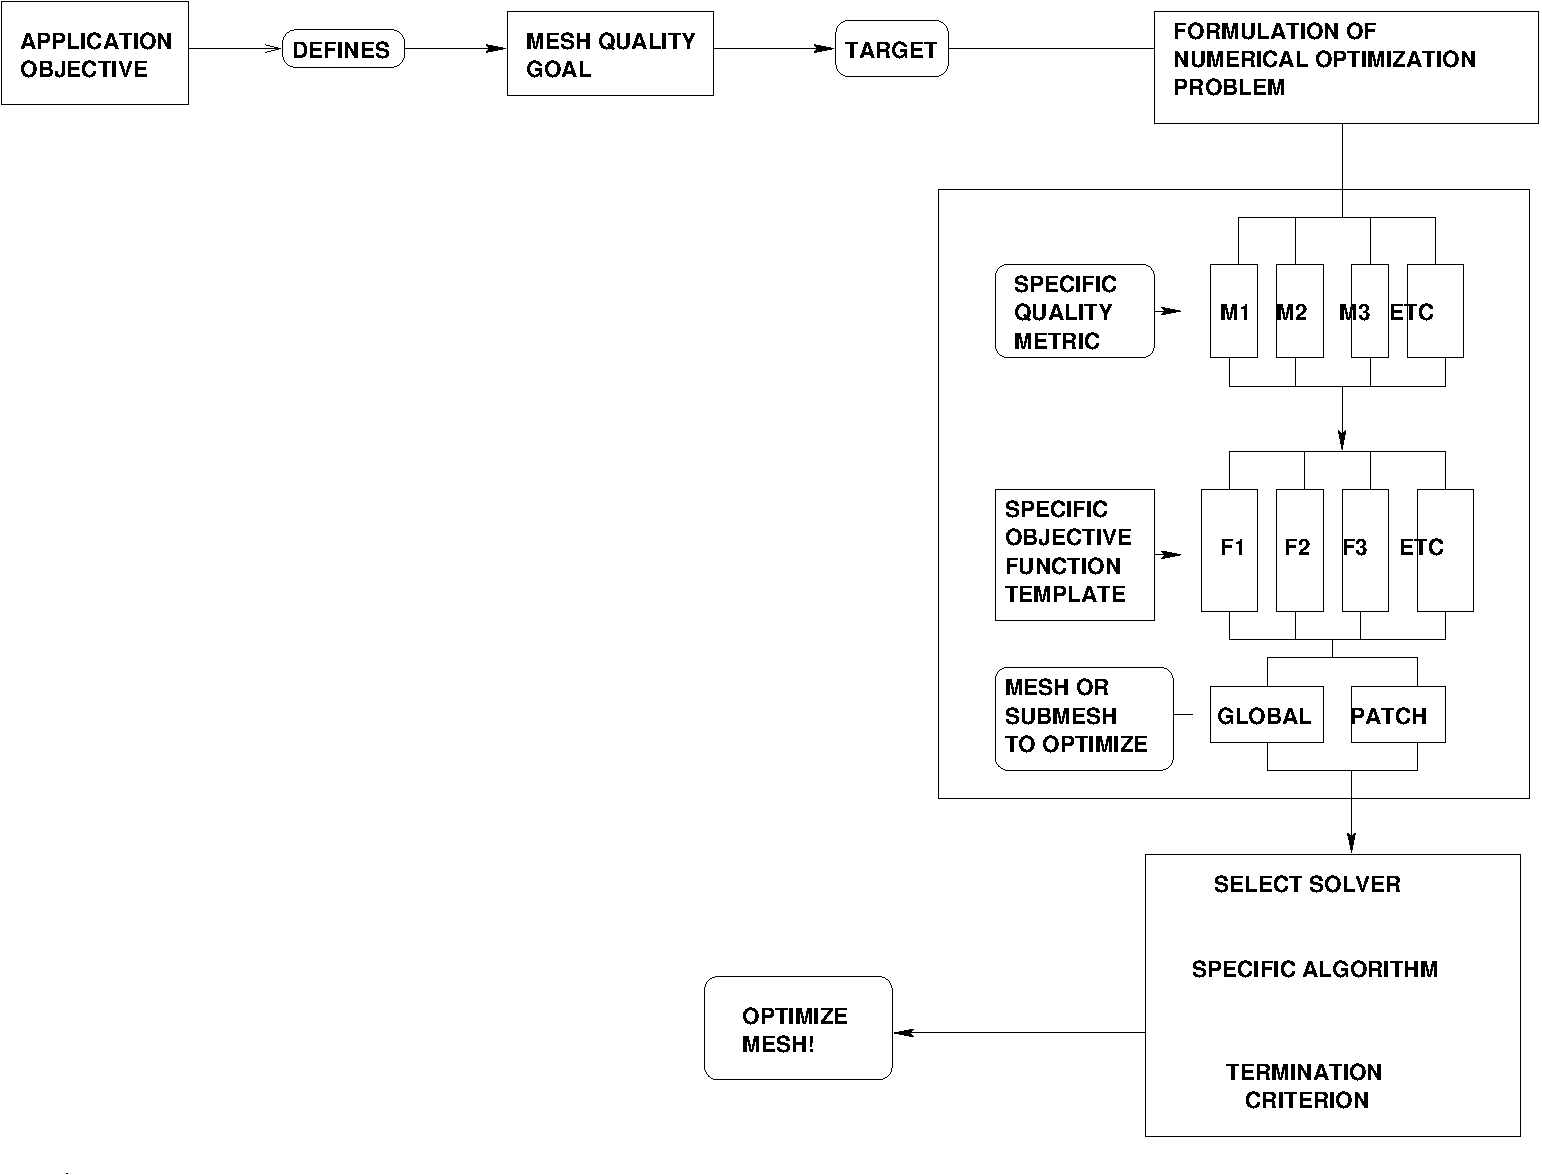
\includegraphics[width=4.7in]{figures/msq-paradigm}
\caption{\em The Mesquite Paradigm \label{Paradigm} }
%\end{tabular}
\end{center}
\end{figure}

\section{How to use this User's Manual}
This user's manual
\begin{itemize}
\item provides an introduction to mesh quality and basic Mesquite concepts (Chapter \ref{sec:intro}),
\item instructs novice users on how to download and install Mesquite (Chapter \ref{sec:install}),
\item provides a tutorial on Mesquite's simplified user's interface and Mesquite's detailed API (Chapter \ref{sec:examples}).
\item describes how to load a mesh in Mesquite via files (Chapter \ref{sec:meshes}), and
%\item provides instructions on using the extensive TSTT interface or a Mesquite mesh specific mesh
%      interface to load a mesh {\it dynamicallu} in Mesquite (sections \ref{sec:msq_mesh}, \ref{sec:TSTT}), and
\item describes Mesquite interactions with domain geometry (Chapter \ref{sec:geom}), and
\item describes Mesquite Wrappers (Chapter \ref{sec:wrappers}),
%\item Exposes in details the concepts and the mechanisms of the advanced API (chapter \ref{sec:API}), and
%\item instructs the user on how to add their own instances of quality
%metrics, objective functions, and solvers (chapter \ref{sec:extensions})
\end{itemize}

Consult the doxygen documentation for the API reference as well as details on the software. There
are two sets of doxygen documentations available:
\begin{itemize}
\item The developer doxygen doc is located in mesquite/doc/developer/. From that directory, you
      must run 'doxygen Mesquite.dox'.
\item The user doxygen doc (API doc) is located in mesquite/doc/user/doxygen. From that directory, you
      must run 'doxygen Mesquite-user.dox'.
\end{itemize}
The doxygen command will generate two directories: an html directory containing the file
index.html that you can open with your web browser, and a latex directory containing a Makefile that
will generate a dvi file.

%\section{Related Documents}

%Documentation of the Mesquite API can be generated from comments in the Mesquite
%source code using the Doxygen utility
%(\url{http://www.stack.nl/~dimitri/doxygen/}).
%To generate HTML and LaTeX copies of this documentation, execute the command
%{\tt doxygen Mesquite-user.dox} in the {\tt doc/usr/doxygen} subdirectory
%of the Mesquite source.

%Further information and related documentation are available on the
%Mesquite home page, located at:
%\url{http://www.cs.sandia.gov/optimization/knupp/Mesquite.html}.
